\subsection{Steered Response Power}

Steered Response Power (SRP) source localization is a method to detect sound source locations using beamforming techniques \cite{krim1996two}. Omologo and Svaizer used the term 'global coherence field' in the 90`s and mapped the level of 'coherence' between two sensors to a source location in space \cite{omologo1994acoustic}. SRP is different from TDOA based methods in that it 'looks' at all possible directions individually (steering) and computes the power of the signal cross correlation in that direction (beamforming). The assumption is that the cross power of the steered microphone array will be the maximum in the correct source direction. The computational demand for this can rise very fast, making it nearly impossible to implement in real time applications. However its performance in difficult conditions outperforms the TDOA based methods \cite{dmochowski2007generalized}. Since real-time localization is not necessary for this thesis, SRP based methods can be considered. In this section, the first part discusses the basic principles behind this method whereas the second part introduces a hybrid method that improves the computational time of SRP without decreasing its robustness.  While the generalized cross correlation is a simple cross correlation between each pair of microphones and only outputs an estimate of the time delay, the SRP method 'beamforms' the space and computes the energy of each location beam. In the same fashion as the GCC method proposed to pre-filter the signal before performing the cross correlation for all the time delay, a PHAT can be applied on the beamformed signal, this method is called SRP-PHAT.

%\subsubsection{Steered Beamformer}

The SRP method is based on a regular delay-and-sum beamformer given by

\begin{equation}
    y_{\rho,\phi,\theta}(n)=\sum\limits_{m=0}^{M-1}{w_m x_m[n + f_{0,m}(\rho,\phi,\theta)]} 
\end{equation}

Where $f_{0,m}(\rho,\phi,\theta)$ is the relative delay from the reference sensor to the $M^{th}$ sensor and $w_m$ is the amplitude weight for that sensor. For $w_m=1$, the output power of the beamformer becomes

\begin{equation}
    \mathbb{E}[{y_{\rho,\phi,\theta}(n)^2}]=\sum\limits_{i=0}^{M-1}\sum\limits_{j=0}^{M-1}{R_{x_i,x_j}[f_{i,j}(\rho,\phi,\theta)]} 
    \label{eq:poweroutputbeamformer}
\end{equation}

Usually cross correlation is computed in the frequency domain using cross-spectrum which is then inverse fast Fourier transformed (IFFT).

\begin{equation}
    R_{x_i,x_j}(\tau)= \sum\limits_{k=0}^{N_{f}-1}{X_{i}(k)X_{j}^*(k)e^{j2\pi\frac{k}{N_{f}}\tau}}
\end{equation}

%\subsubsection{SRP Search}

The SRP method starts with a look up procedure which associates each set of coordinate ($\rho,\phi,\theta$) to a given set of delays between each microphone pair. For instance, if we do not care about the range and use a 1 degree resolution, the SRP method associates 360*360=129600 angular positions to corresponding delays. The cross correlations at the particular delay are then computed. When the beamforming of the space and the computation of the cross correlation are completed the angular position that gives the maximum value at the beamformer output is chosen as an estimate of the main source location in the case of single source detection. For multiple sources, local maxima can also be selected. For a given position, the output of the SRP search is the sum of the cross correlation at each time delay found relative to each pair of microphone. It corresponds to the power output of the beamformer defined in equation \ref{eq:poweroutputbeamformer}
\begin{equation}
    S^{SRP}(\rho,\phi,\theta)=\sum\limits_{i=0}^{M-1}\sum\limits_{j=0}^{M-1}{R_{x_i,x_j}[f_{i,j}(\rho,\phi,\theta)]}
\end{equation}

The SRP method estimates the source location ($\Hat{\rho},\hat{\phi},\hat{\theta}$) after creating the SRP search space such that

\begin{equation}
    (\Hat{\rho},\hat{\phi},\hat{\theta})=\argmax_{\rho,\phi,\theta}S^{SRP}(\rho,\phi,\theta)
\end{equation}

%\subsubsection{Premapping the delays to potential sources locations}

The classical SRP search beamforms sequentially the 3D space and locations [($\rho_{1},\phi_{1},\theta_{1}$), ($\rho_{2},\phi_{2},\theta_{2}$), ... ,($\rho_{x},\phi_{x},\theta_{x}$)] which might be associated with the same relative delays $\tau_{1}$. The cross correlation at delay $\tau_{1}$ is then computed $x$ times, which lead to the same results for each [($\rho_{1},\phi_{1},\theta_{1}$), ($\rho_{2},\phi_{2},\theta_{2}$), ... ,($\rho_{x},\phi_{x},\theta_{x}$)] positions, leading to numerous useless cross correlation computations. In \cite{dmochowski2007generalized} the authors propose an improvement on the SRP search algorithm by pre-mapping the relative delays to their corresponding set of locations. Instead of proceeding to a sequential search in the 3D space, a search on the relative possible delays is considered. The possible delays between individual microphone pairs are already known based on the array geometry and can be stored in memory. The cross correlations are calculated for each delay subset and related a set of potential source location in space in the final steps of the algorithm. Note that the computational cost gain can be immense depending on the number of microphones (the more the microphones, the greater the gain). Care should be taken if the array has a large aperture and is therefore subject to spatial aliasing. Pre-filtering the signal beforehand by using PHAT introduces a function $\psi_{ij}$ in the cross correlation

\begin{equation}
    R_{x_i,x_j}(\tau)= \sum\limits_{k=0}^{N_{f}-1}{\psi_{ij}(k) X_{i}(k)X_{j}^*(k)e^{j2\pi\frac{k}{N_{f}}\tau}}
\end{equation}
where
\begin{equation}
    \psi_{ij}(k) = \frac{1}{|{X_{i}(k)X_{j}^*(k)}|}
\end{equation}

\subsubsection{Hybrid SRP-PHAT}

In \cite{peterson2005hybrid} the author describes a novel approach for sound localization using a two stage approach in order to reduce the computational load. The first stage identifies roughly the sources locations while the second stage is a modified version of the SRP-PHAT algorithm that only performs a grid search around the estimated location from the first stage.  The method described in \cite{peterson2005hybrid} is well suited for near-field location using large aperture array which is not our requirement but the idea can be adapted in the case of far-field sound localization. Section \ref{sec:TDOA} gives an introduction to TDOA based localization and introduces the cone approximation for the far-field. The idea of the hybrid approach is to do a classical GCC-PHAT estimation to get the relative delays between the sensors. The delays estimates are used to derive the cone intersections which give a location estimate which is then inputted into a SRP-PHAT algorithm where the search region is constrained around the location estimates. A system overview of the algorithm is given in figure \ref{fig:hybridalgo}.

\begin{figure}[H]
    \centering
    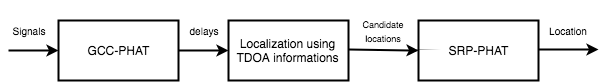
\includegraphics[width=1\textwidth]{Figures/hybridalgo.png}
    \caption{Simplified block diagram of the Hybrid algorithm}
    \label{fig:hybridalgo}
\end{figure}

\subsubsection{Improvements on SRP}

In \cite{salvati2017exploiting} the author proposes a method to improve the computational efficiency and coherence of the grid search using discreet sampling information where the method is called geometrically sampled grid (GSG). \cite{do2007real} uses Stochastic Region Contraction(SRC) to reduce the computational time of the search. \cite{salvati2014incoherent} introduces an incoherent Frequency Fusion based on a normalized arithmetic mean (NAM) which improves the localization performance of SRP, MVDR and MUSIC. Paper \cite{salvati2015frequency} introduces a SRP weighted MVDR, which combines machine learning power to the noise resilience of the MVDR beamformer, the method is improved in \cite{salvati2016use} by using SVM training. SRP-WMVDR is proved to be much more resilient to noise and better than SRP-PHAT for SNR up to 0. All of those papers uses a microphone array composed of mostly more than 8 microphones. Few experiment data are available for the case of 4 microphones and none for the case of a tetrahedral array, whereby a ULA is mostly used for the different test methods.


